\documentclass[00_complete]{subfiles}

%\documentclass[12pt]{report}
\usepackage[utf8]{inputenc}
\usepackage{amsmath,amssymb,amsthm,gensymb,parskip,graphicx,footmisc,csquotes,enumerate,datetime2}
\usepackage[]{libertinus}
\usepackage[breaklinks]{hyperref}
\hypersetup{
  pdfauthor={Moshe Krumbein},
  colorlinks=true,
  linkcolor={black},
  filecolor={black},
  citecolor={black}, %blue
  urlcolor={black}, %blue
}
\usepackage[top=30mm,bottom=30mm,left=30mm,right=30mm]{geometry}
%\setlength{\emergencystretch}{2em} % prevent overfull lines
\providecommand{\tightlist}{%
\setlength{\itemsep}{0pt}\setlength{\parskip}{0pt}}

\renewcommand\qedsymbol{$\blacksquare$}

\theoremstyle{definition}
\newtheorem*{definition}{Definition}
\newtheorem*{theorem}{Theorem}
\newtheorem*{axiom}{Axiom}
\newtheorem*{lemma}{Lemma}

\theoremstyle{remark}
\newtheorem*{note}{Note}
\newtheorem*{symbols}{Symbol}
\newtheorem{example}{Example}[section]
\newtheorem*{claim}{Claim}
\newtheorem*{conclusion}{Conclusion}
\newtheorem*{reminder}{Reminder}

\usepackage{fancyhdr}
\usepackage[italicdiff]{physics}
\MakeOuterQuote{"}

\renewcommand{\chaptermark}[1]{\markboth{#1}{}}

\pagestyle{fancy}

\setlength{\headheight}{14.5pt}
\addtolength{\topmargin}{-2.5pt}

\fancyhf{}
\rhead{Moshe Krumbein}
\lhead{\chaptermark}
\cfoot{\thepage}
\fancyhead[R]{\chaptername~\thechapter}
\fancyhead[L]{\mbox{\leftmark}}

\usepackage[Rejne]{fncychap}
\usepackage{titling}

\makeatletter
\renewcommand{\@chapapp}{\vspace*{-100pt}\huge\thetitle}
\makeatother

\makeatletter
\newcommand{\subtitle}[1]{%
  {\center\vspace*{-60pt}%
  \linespread{1.1}\Large\scshape#1%
  \par\nobreak\vspace*{35pt}}
}
\makeatother

\newcommand{\Chapter}[2]{
    \def\n{#2}
    \setcounter{chapter}{\the\numexpr\n-1}
    \chapter{#1}
    \subtitle{\theauthor~- \thedate}
}

\DeclareMathOperator{\Ima}{Im}
\DeclareMathOperator{\Id}{Id}
\DeclareMathOperator{\cis}{cis}

\newcommand{\Mod}[1]{\ (\mathrm{mod}\ #1)}
\newcommand{\st}[0]{\;\mathrm{s.t.}\;}

\title{Discrete Mathematics}
\author{Moshe Krumbein}
\date{Fall 2021}

\begin{document}
\Chapter{The Pigeonhole Principle and Induction}{8}

\section{The Pigeonhole Principle}
\subsection{Definition and Examples}
\begin{definition}[The Pigeonhole Principle]
    Given $m, n \in \mathbb{N}, m>n$, then if we distribute $m$ pigeons between
    $n$ pigeonholes, then at least one hole with have at least two pigeons.

    In other words, if $m>n$, then there does not exist $f: [m] \to [n]$ that
    will be \emph{injective}.
\end{definition}

\begin{claim}[First Example]
    Suppose $A =\{0,1,2,\dots,11\}$. If we choose $7$ numbers within $A$ then
    we are guaranteed that there will be two numbers from our choice that will
    add to $11$.
\end{claim}

\begin{proof}
    We define the following $6$ sets:
    $$\{0,11\},\{1,10\}, \{2,9\}, \{3,8\}, \{4,7\}, \{5,6\}$$
    where the sum of the elements of the set is equal to $11$.

    According to the \emph{pigeonhole principle}, if we pick $7$ numbers, we
    will certainly pick at least one of the $6$ previously mentioned sets.
\end{proof}

\begin{claim}[Second Example]
    If we choose $101$ numbers from the set $\{1,2,\dots,200\}$, we can be
    guaranteed that among the numbers we picked, one will divide
    another.
\end{claim}

\begin{proof}
    For all $1 \leq i \leq 100$, we define:
    $$B_i=\{2i-1,2i\} \quad \bigcup_{i=1}^{100}B_i=[200]$$
    \begin{reminder}
        For all $n \in \mathbb{N}$, there exists a single prime factorization
        and specifically for $n \in [200]$, there exists $a_n,b_n$ such that:
        $$n=2^{a_n}\cdot b_n$$
        where $a_n \in \mathbb{N} \cup \{0\}, b_n \in \mathbb{N}$.
    \end{reminder}
        We notice that if $n \in [200]$ then $1 \leq b_n \leq 200$, or in other
        words: $b \in \{1,3,5,\dots,199\}$.

        For all $j \in \{1,3,5,\dots,199\}$ we define:
        $$B_j = \{n \in [200] \mid n=n^m \cdot j\}$$
        In other words, the only odd factor in $B_j$ will be $j$ itself.
        \begin{enumerate}
            \item From the singularity of prime factorization:
                $$j_1 \neq j_2 \implies B_{j_1}\cap B_{j_2}=\emptyset$$
            \item
                $$\bigcup_{j \in \{1,3,5,\dots,199\}}B_j=[200]$$
            \item If $k,l \in B_j$ then we are guaranteed that one will divide
                another: (without loss of generality: $n_1 < n_2$)
                $$
                \begin{gathered}
                    k=2^{n_1}\cdot j \quad l=2^{n_2} \cdot j \\
                    2^{n_1}j|2^{n_2}j \implies k|l
                \end{gathered}
                $$
        \end{enumerate}
\end{proof}

\begin{claim}[Third Example]
    Between all $n+1$ different natural numbers, we can find $2$ numbers such that
    their difference divides $n$ without a remainder.
\end{claim}

\begin{proof}
    \begin{reminder}
        We have see that relation over the natural number defined as:
        $$a \sim b: a-b=0\Mod{n}$$
    \end{reminder}
    Given $n+1$ different natural numbers, as per the \emph{pigeonhole
    principle}, $2$ are part of the same \emph{equivalence class}.
\end{proof}

\begin{claim}[Fourth Example]
    If $13$ natural numbers are written in a row, then there exists a run of
    adjacent numbers such that their sum divides by $13$.
\end{claim}
\begin{proof}
    We define $1\leq k \leq 13$ such that:
    $$b_k=\sum_{i=1}^{k}a_i \quad b_{0}=0$$
    From the previous claim, there exists $0 \leq i<j \leq 13$ such that:
    $$b_j-b_i=0\Mod{13}$$
    However:
    $$b_j-b_i = \sum_{k=i+1}^{j}a_k$$
    $$b_j-b_i=(a_1+a_2+\dots+a_j)-(a_1+a_2+\dots+a_i)=a_{i+1}+a_{i+2}+ \dots + a_j$$
\end{proof}
\subsection{Erd\H{o}s–Szekeres theorem}
\begin{definition}[Erd\H{o}s–Szekeres theorem]
    Sequence $(a_1,\dots,a_n)$ is \emph{monotonic} if $a_1 \leq a_2 \leq \dots
    \leq a_n$ or $a_1 \geq a_2 \geq \dots \geq a_n$

    Given sequence $A=(a_1,a_2,\dots,a_n)$, if $1 \leq i_1 \leq i_2 \leq \dots
    leq i_k \leq k$ of $k$ natural numbers, then $(a_{i_1}, a_{i_2}, \dots
    a_{i_k})$ is a \emph{subsequence} of length $k$ of $A$.

    Given series of $nm+1$ distinct numbers then there exists a subsequence
    either \emph{increasing} with length $n+1$ or \emph{decreasing} with the
    length $m+1$.
\end{definition}
\begin{example}[Erd\H{o}s–Szekeres theorem]
    $$
    \begin{gathered}
        (1,5,0,3,2) \\
        \text{Length of: } 2 \cdot 2 + 1 \\
        \text{There is a decreasing subsequence of length: } 2+1
    \end{gathered}
    $$
\end{example}
\begin{conclusion}
    For every sequence of the length $1\cdot 11 + 1 = 12$ we can find a
    decreasing subsequence of length $2$ or an increasing subsequence of length
    $2$.
\end{conclusion}
\begin{proof}
    We define of all $i: 1 \leq i \leq nm+1$:

    $p_1$ - length of increasing subsequence with maximum length beginning with
    $a_i$.

    $q_1$ - length of decreasing subsequence with maximum length beginning with
    $a_i$.

    \emph{Proof by contradiction}: there does not exist a subsequence with length
    $m+1$, then for all $i: 1 \leq p_i \leq m$.

    If there also isn't a decreasing subsequence with a length $n+1$ then for
    all $i: 1 \leq q_i \leq n$.

    Therefore, for all $1 \leq i \leq nm+1$:
    $$
    \begin{gathered}
        (p_i,q_i) \in [m] \times [n] \\
        |[m] \times [n]| = mn
    \end{gathered}
    $$
    We have $nm+1$ ordered pairs that are each part of a set with the size
    $nm$.

    Per the \emph{pigeonhole principle}, there exists $1\leq i<j \leq nm+1$
    such that $(p_i,q_i)=(p_j,q_j)$. However, we know that $a_i \neq a_j$.

    If $a_1<a_j$, then $p_i>p_j$, which is a contradiction.

    If $a_1>a_j$, then $p_i<p_j$, which is a contradiction.
\end{proof}

\subsection{Generalized Pigeonhole Principle}

If we distribute $ab+1$ pigeons in $a$ holes, then there is a hole that has at
least $b+1$ pigeons.

\begin{proof}
    We will prove \emph{by contradiction}:

    We define $c_i$ as the number of pigeons that come from the
    $i^{\mathrm{th}}$ hole.

    According to the negative assumption, for all $i$, $c_i \leq b$, where we
    receive:
    $$ab+1=\sum_{i=1}^{a}c_i\leq \sum_{i=1}^{a}b = ab$$
    Which is a contradiction.
\end{proof}

\begin{example}
    For every group of 6 people, we will be able to find either 3 people
    who know one another or 3 people who do not know one another.
\end{example}
\begin{proof}
    Suppose \emph{Dani} is one of the people in a group.

    Everyone else in the group can be split up into one of two groups:
    \begin{itemize}
        \item[A -] People who know \emph{Dani}.
        \item[B -] People who don't know \emph{Dani}.
    \end{itemize}
    Per the \emph{generalized pigeonhole principle}, there will be a group
    containing 3 people.

    If $|A|\geq 3$, if among set $A$ there are at least 2 people who know each other, then along
    with \emph{Dana}, we will find 3 people in the group who know one
    another. If there aren't, then we know there are 3 people in set $A$ who do
    not know one another.

    Similarly, if $|B|\geq3$, if they don't know one another then there are 3
    people know don't know each other and if they all know each other then that
    satisfies the requirement of having three people know each other.
    $$5=\underbrace{2}_{a}\cdot\underbrace{2}_{b}+1$$
\end{proof}

\begin{example}
    A plane is colored with the colors green and white. Is is guaranteed that
    we will be able to find two \emph{monochromatic} (the same color) points
    such that the distance between them is exactly $1$m?
    \begin{proof}
    Consider the vertices of an equilateral triangle of side length 1 on the
    plane. Per the \emph{pigeonhole principle} at least two of the vertices
    will be the same color.
\end{proof}
    If we go up a dimension and consider a swimming pool colored with 3
    different colors, we will still be able to find two monochromatic points at
    distance $1$m from one another if we consider \emph{tetrahedron}
    (three-sided pyramid) instead of a triangle in our previous proof.
\end{example}

\section{Induction}

\subsection{What is induction?}
A proof technique regarding the natural numbers.

\begin{axiom}[Axiom of Induction]
    For all $\emptyset \neq A \subseteq \mathbb{N}$, there exists a \emph{minimum
    term}.

    In other words:
    $$\exists a_0 \in A \st \forall a \in A: a_0 \leq a$$
\end{axiom}

Method of proving $p(n)$ using induction over the real numbers:
\begin{enumerate}[I.]
    \item \emph{Base case of induction}.

    To show the statement holds for $p(1)$.
    \item \emph{Induction step}.

    Posits that if $p(k)$ is true ($p \in \mathbb{N}$), then $p(k+1)$ will also
    be true.
\end{enumerate}
If both steps are true, we can deduce that for $n in \mathbb{N}$, $p(n)$ is true.
\begin{proof}
    We will assume by counterexample that the two steps are true but not for
    all $n \in \mathbb{N}$, $p(n)$ is true.

    We define $A =\{n \mid p(n) \text{ is false}\} \subseteq \mathbb{N}$, and
    According to our assumption, $A \neq \emptyset$. As per the \emph{axiom of
    induction}, there exists $n_0 = \min{A}$. We know that $1 \notin A$ and
    therefore $n_0>1$, $n_0-1 \notin A$, $n_0-1 \in \mathbb{N}$ and therefore
    $p(n_0-1)$ is true. Per \emph{induction}, $p(n_0)$ must also be true, which
    is a contradiction.
\end{proof}
\subsection{Examples}
\setcounter{example}{0}
\begin{example}
    $$1+3+5+\dots+(2n+1)= \sum_{k=1}^{n}(2k-1)=n^2$$
\begin{proof}
    \begin{enumerate}[I.]
        \item $p(1)$:
        \begin{equation}
        1= \sum_{k=1}^{1}2k-1 =1 \tag{\checkmark}
        \end{equation}
        \item \emph{Induction step}

        Let's suppose $p(j)$ and prove $p(j+1)$.
        \begin{gather*}
            \sum_{k=1}^j(2k-1)=j^2 \\
            \sum_{k=1}^{j+1}(2k-1)=(j+1)^2 \\
            \sum_{k=1}^{j+1}(2k-1) = \sum_{k=1}^j(2k-1)+2(j+1)-1 = j^2+2j+1 =
            (j+1)^2 \tag{\checkmark}
        \end{gather*}
    \end{enumerate}
\end{proof}
\end{example}
\begin{example}
    For all $n \in \mathbb{N}$, $3|4^n-1$.
    \begin{proof}
    \begin{enumerate}[I.]
        \item
            \begin{equation}
                3|4^1-1 \tag{\checkmark}
            \end{equation}
        \item
            \begin{gather*}
                \exists t \in \mathbb{Z} \st 4^k-1=3t \\
                4^{k+1}-1=4\cdot 4^k-1 = 3\cdot 4^k + 4^k-1=3\cdot
                4^k+3t=3(4^k+1) \\
                4^k+1 \in \mathbb{Z} \implies 3|4^{k+1}-1\tag{\checkmark}
            \end{gather*}
    \end{enumerate}
    \end{proof}
\end{example}
\begin{example}
    For all $n \in \mathbb{N}$ it is possible to tile a grid of the size $2^n
    \times 2^n$ (excluding a $1 \times 1$ corner square) with "L" tiles (or any
    rotation of an "L" tile).
\begin{figure}[ht]
  \centering
    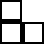
\includegraphics[width=0.1\textwidth]{w8_l}
    \caption{"L" tile}
\end{figure}
\begin{proof}
    \begin{enumerate}[I.]
        \item
        \begin{equation}
            2^1 \times 2^1 - \text{ just place one "L" piece}
            \tag{\checkmark}
        \end{equation}
        \item
        $2^k \times 2^k$ works.

        Given $2^{k+1} \times 2^{k+1}$, we can divide it into 4 smaller square
        of $2^k \times 2^k$.
    \end{enumerate}
\end{proof}
\end{example}
\subsection{Expansion on Induction}
\setcounter{example}{0}
\begin{theorem}[Expansion of Induction]
    Given $p(n), n \in \mathbb{N}$:
    \begin{enumerate}[I.]
        \item $p(n_0)$ is true for $n_0 \in \mathbb{N}$
        \item $p(k)\implies p(k+1)$
    \end{enumerate}
    Therefore, for all $n \in \mathbb{N}$ such that $n \geq n_0$, $p(n)$ is
    true.
\end{theorem}
\begin{theorem}[Complete Induction]
    Given $p(n)$ over the natural numbers:
    \begin{enumerate}[I.]
        \item $p(1)$ is true.
        \item $p(1)\land p(2) \land \dots \land p(k) \implies p(k+1)$
    \end{enumerate}
\end{theorem}
\begin{example}
    For all $n \in \mathbb{N}$, $n$ can be expressed as a product of prime
    numbers.
    \begin{proof}
        \begin{enumerate}[I.]
            \item $p(1)$: $1$ is a multiple of $0$ primes.
            \item Assuming $p(1), p(2), \dots, p(k)$:

                If $k+1$ is prime, we're done.

                If not, then there exists $b,c \in \mathbb{N} \setminus \{1\}$
                such that $bc=k+1$. Since $b,c < k+1$ through \emph{complete
                induction}, we know that both $b$ and $c$ can be expressed as a
                product of primes, and therefore we see that $k+1$ can be
                expresses as the product of $b$ and $c$'s prime factors.
        \end{enumerate}
    \end{proof}
\end{example}
\begin{example}
    For all $n \in \mathbb{N}$, there are $n$ prime numbers.
    \begin{proof}
        \begin{enumerate}[I.]
            \item \begin{equation}
                n=1 \tag{\checkmark}
            \end{equation}
            \item We suppose there exists $k$ primes $p_1,p_2,p_3,\dots
                p_k$ and we'll prove that there exists $k+1$ primes.

                Consider $q=p_1\cdot p_2 \cdot \ldots \cdot p_k+1$.

                $q$ isn't divisible by $p_1,p_2,\dots p_k$.

                If $q$ is prime, we're done.

                If $q$ isn't prime, it still must have a prime factor, but
                since $q$ isn't divisible by $p_1,p_2,\dots p_k$, we know there
                are at least $k+1$ primes.
        \end{enumerate}
    \end{proof}
\end{example}
\end{document}
